\documentclass{article}
\title{Stockfish chess statistics}
\author{Johan Bjerkem}
\usepackage{multirow}\usepackage{pgfplots}\begin{document}
\maketitle
In this document i will present tables, graphs and statistics about 2600 chess games played by the chess engine Stockfish. The game information is gathered from the document 'Stockfish\textunderscore15\textunderscore64-bit.commented.[2600].pgn'. Hopefully you find the data insightful.\\\\First we will have a look at the win, loss and draw statistics for Stockfish. The data is presented in a table, where you also can read what color Stockfish played as.
\begin{center}
\begin{tabular}{l|rrr}
Color/Result & Wins & Draws & Losses\\
\hline
Any & 992 & 1600 & 8\\
White & 698 & 601 & 2\\
Black & 294 & 999 & 6\\
\end{tabular}
\end{center}

Below is a graph showing the number of games that is still active after $x$ number of moves.

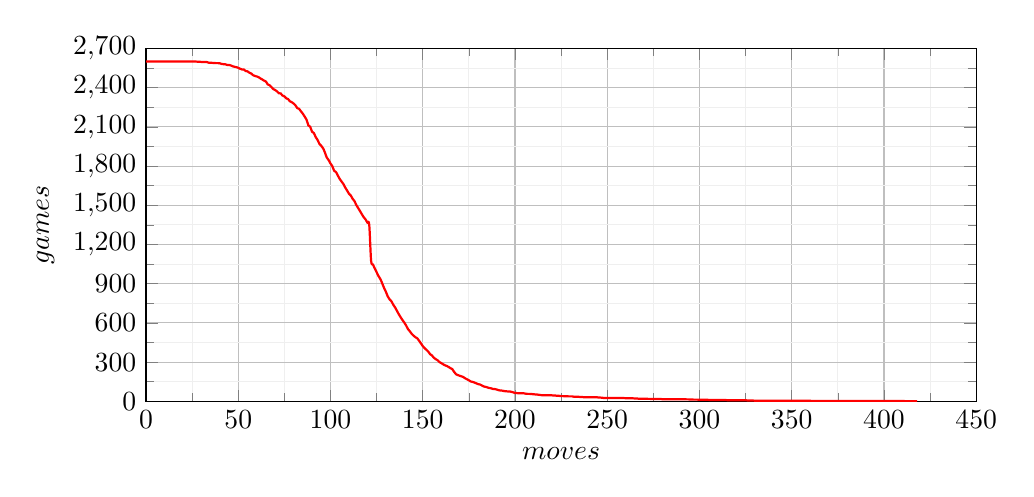
\begin{tikzpicture}
\begin{axis}[
	xmin = 0, xmax = 450,
	ymin = 0, ymax = 2700,
	xtick distance = 50,
	ytick distance = 300,
	grid = both,
	minor tick num = 1,
	major grid style = {lightgray},
	minor grid style = {lightgray!25},
	width = \textwidth,
	height = 0.5\textwidth,
	xlabel = {$moves$},
	ylabel = {$games$},]
\addplot[
	smooth,
	thick,
	red,
]
coordinates {
(0,2600)(1,2600)(2,2600)(3,2600)(4,2600)(5,2600)(6,2600)(7,2600)(8,2600)(9,2600)(10,2600)(11,2600)(12,2600)(13,2600)(14,2600)(15,2600)(16,2600)(17,2600)(18,2600)(19,2600)(20,2600)(21,2600)(22,2600)(23,2600)(24,2600)(25,2600)(26,2600)(27,2600)(28,2599)(29,2599)(30,2597)(31,2597)(32,2596)(33,2596)(34,2591)(35,2591)(36,2590)(37,2589)(38,2588)(39,2588)(40,2587)(41,2582)(42,2580)(43,2579)(44,2574)(45,2574)(46,2570)(47,2564)(48,2560)(49,2557)(50,2552)(51,2545)(52,2540)(53,2539)(54,2528)(55,2525)(56,2515)(57,2509)(58,2496)(59,2490)(60,2486)(61,2481)(62,2471)(63,2463)(64,2454)(65,2447)(66,2425)(67,2419)(68,2405)(69,2389)(70,2382)(71,2372)(72,2358)(73,2356)(74,2340)(75,2334)(76,2319)(77,2313)(78,2296)(79,2289)(80,2279)(81,2265)(82,2244)(83,2238)(84,2219)(85,2201)(86,2179)(87,2156)(88,2112)(89,2101)(90,2063)(91,2053)(92,2021)(93,2000)(94,1970)(95,1955)(96,1936)(97,1903)(98,1865)(99,1846)(100,1820)(101,1799)(102,1764)(103,1754)(104,1727)(105,1702)(106,1682)(107,1663)(108,1636)(109,1613)(110,1589)(111,1575)(112,1550)(113,1532)(114,1502)(115,1479)(116,1456)(117,1432)(118,1409)(119,1392)(120,1368)(121,1351)(122,1077)(123,1047)(124,1017)(125,988)(126,959)(127,937)(128,904)(129,869)(130,839)(131,804)(132,781)(133,766)(134,740)(135,719)(136,693)(137,667)(138,644)(139,622)(140,603)(141,580)(142,553)(143,536)(144,517)(145,503)(146,491)(147,483)(148,464)(149,444)(150,423)(151,407)(152,394)(153,380)(154,361)(155,351)(156,334)(157,323)(158,315)(159,301)(160,293)(161,284)(162,276)(163,271)(164,263)(165,254)(166,247)(167,226)(168,208)(169,201)(170,196)(171,191)(172,186)(173,176)(174,169)(175,161)(176,152)(177,149)(178,144)(179,138)(180,132)(181,129)(182,122)(183,114)(184,111)(185,107)(186,102)(187,100)(188,95)(189,94)(190,91)(191,86)(192,83)(193,82)(194,79)(195,77)(196,76)(197,76)(198,73)(199,69)(200,64)(201,63)(202,62)(203,62)(204,62)(205,61)(206,58)(207,57)(208,57)(209,56)(210,54)(211,53)(212,52)(213,50)(214,48)(215,46)(216,46)(217,46)(218,46)(219,46)(220,46)(221,44)(222,44)(223,42)(224,42)(225,40)(226,40)(227,39)(228,39)(229,38)(230,38)(231,38)(232,35)(233,35)(234,35)(235,34)(236,34)(237,32)(238,32)(239,32)(240,32)(241,32)(242,32)(243,32)(244,32)(245,30)(246,29)(247,28)(248,26)(249,26)(250,26)(251,26)(252,25)(253,25)(254,25)(255,25)(256,25)(257,25)(258,25)(259,25)(260,24)(261,24)(262,23)(263,23)(264,23)(265,22)(266,22)(267,20)(268,20)(269,20)(270,20)(271,20)(272,19)(273,19)(274,18)(275,18)(276,18)(277,18)(278,18)(279,18)(280,16)(281,16)(282,16)(283,16)(284,16)(285,16)(286,16)(287,16)(288,16)(289,16)(290,16)(291,16)(292,16)(293,15)(294,15)(295,14)(296,14)(297,13)(298,13)(299,13)(300,12)(301,12)(302,12)(303,12)(304,12)(305,11)(306,11)(307,11)(308,11)(309,11)(310,11)(311,10)(312,10)(313,10)(314,10)(315,9)(316,9)(317,8)(318,8)(319,8)(320,8)(321,8)(322,8)(323,8)(324,8)(325,8)(326,7)(327,7)(328,6)(329,6)(330,5)(331,5)(332,5)(333,5)(334,5)(335,5)(336,5)(337,5)(338,5)(339,5)(340,5)(341,5)(342,5)(343,5)(344,5)(345,5)(346,5)(347,5)(348,5)(349,4)(350,4)(351,4)(352,4)(353,4)(354,4)(355,4)(356,4)(357,4)(358,4)(359,4)(360,4)(361,3)(362,3)(363,3)(364,3)(365,3)(366,3)(367,3)(368,3)(369,3)(370,3)(371,3)(372,3)(373,3)(374,3)(375,3)(376,3)(377,3)(378,3)(379,3)(380,3)(381,3)(382,3)(383,3)(384,3)(385,3)(386,3)(387,3)(388,3)(389,3)(390,3)(391,3)(392,2)(393,2)(394,2)(395,2)(396,2)(397,2)(398,2)(399,2)(400,2)(401,2)(402,2)(403,2)(404,2)(405,2)(406,2)(407,2)(408,2)(409,2)(410,2)(411,2)(412,1)(413,1)(414,1)(415,1)(416,1)(417,1)(418,1)
};
\end{axis}
\end{tikzpicture}
\end{document}
